\documentclass[a4paper,english, 11pt]{article}

\usepackage[a4paper,inner=2.5cm,outer=2.5cm,top=2.5cm,bottom=2.5cm,pdftex]{geometry} 
\usepackage{graphicx}
\usepackage{titling}
\usepackage[colorlinks = true,
            linkcolor = blue,
            urlcolor  = blue,
            citecolor = blue,
            anchorcolor = blue]{hyperref}
\usepackage{enumerate}
\usepackage{fancyhdr}
\usepackage{lastpage}
\usepackage{booktabs} % For better table formatting
\usepackage{array} % for the 'p' column type
\hypersetup{colorlinks=true,linkcolor=blue, linktocpage}

\newcommand{\emailme}{\href{mailto:lukem@unis.no}{lukem@unis.no}}

% header
\pagestyle{fancy}
\fancyhf{}
\fancyhfoffset[L]{1cm} % left extra length
\fancyhfoffset[R]{1cm} % right extra length
\rhead{\today}
\lhead{\bfseries UNIS data management plan}
% footer
\rfoot{page \thepage\ of \pageref*{LastPage}}

% title
\title{How to create a Darwin Core Archive}
\date{\today}
\author{Luke Marsden (\emailme)}

\begin{document}

\maketitle
\tableofcontents
\newpage

\section{What is a Darwin Core}
\label{s:dwc}

Darwin Core is a data standard originally developed for biodiversity informatics, though this has expanded to be useful for any type of data where you have data associated with one or a list of organisms. Darwin Core includes
\begin{itemize}
\item Darwin Core terms: A controlled vocabulary of terms - \url{https://dwc.tdwg.org/terms/}
\item Darwin Core Archive: A FAIR data format
\end{itemize} 

\section{What is a Darwin Core Archive}
\label{s:dwca}

A Darwin Core Archive (DwCA) is a self-describing dataset for taxonomic (species) data and sampling event data. It consists or one or more data tables (CSV files) and 2 XML files, one (meta.xml) that describes how the files are organised and a second  (eml.xml) that provides the metadata describing the dataset as a whole. They are zipped together to create the Darwin Core Archive (DwCA) (Figure \ref{fig:dwca}). 

Each CSV file contains a number of rows, and every row has its own unique ID. These IDs are used to link the CSV files together. Every row in every `extension' CSV file must include the ID of one row in the `core' CSV file. This is called the `star schema' and you can think of the core as the centre of the star. Note that a DwCA can only include a single `level' of extensions. In other words, it cannot include an extension to an extension file.


It has a single core in the centre of the star, for example event records, where a single row corresponds to a single event. 
Each row has its own ID.  
This central core can then optionally be surrounded by extension tables, linked to the central core using this ID. 

\begin{figure}[htb]
    \tcbox[colback=white]{
    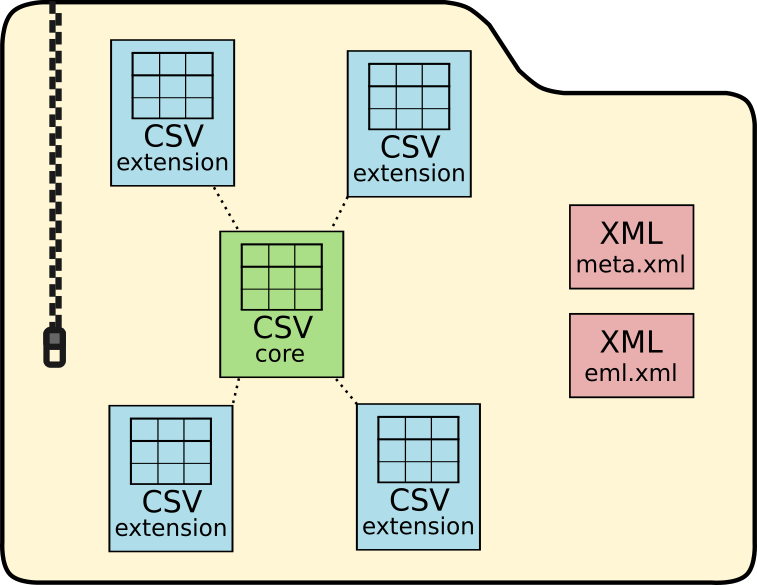
\includegraphics[width=0.7\textwidth]{dwca.png}
    }
    \caption{\label{fig:dwca}
        Visualisation of a Darwin Core Archive, portrayed using the star schema. The
        central event core can be surrounded by zero or many extension tables.
        It also contains a meta.xml file that describes what columns each CSV contains and links them to the term in a controlled volcabulary, and an eml.xml file that provides metadata that describes the dataset as a whole. They are zipped together to create a Darwin Core Archive.
    }
\end{figure}

For more information on DwCA, see \url{https://ipt.gbif.org/manual/en/ipt/2.5/dwca-guide}.


\subsection{Why do we use multiple CSV files?}
\label{ss:multiplefiles}

This is a common question, but we are not trying to make things needlessly complicated! This allows a many-to-one relationship to be logged, for example multiple species (occurrences) logged for a single sampling event. Hierarchical information can be stored clearly, so the data user can understand which samples were collected from the same sampling event.

This method is also more efficient. Certain metadata are consistent between the sampling event and all the samples collected from it, e.g. time, date, coordinates etc. These metadata can be logged only once for each sampling event in an event core. They therefore do not need to be included for every single sample, which would lead to a lot of duplication in some cases!

\section{Darwin Core terms and other controlled vocabularies}
\label{s:dwcterms}

Darwin Core includes a controlled vocabulary of terms for sharing information about biological diversity. Most (but not all) of the column headers you will include in your CSV files in your DwCA will be Darwin Core terms. Other terms will be from other controlled vocabularies.

We will come back to which terms you should include later.

\section{GBIF, OBIS and a network of data}
\label{s:gbif}

There are a number of data centres and services that manage Darwin Core data. GBIF (Global Biodiversity Information Facility) is the largest. Most (all?) of the other Darwin Core services make their data available via GBIF as well as their own platform. So if you publish your data with any of the below services, your data will also be available via GBIF.

\begin{table}[h!]
\centering
\caption{A network of Darwin Core data. This table is just a small selection of the services available.}
\begin{tabular}{cp{6cm}p{6.5cm}}
\toprule
Name & Website       & Comment  \\
\midrule
OBIS       & \url{https://obis.org/} & Only marine data. The OBIS community have been pushing the DwC standards forwards to build better functionality for scientific data.      \\
iNaturalist       & \url{https://www.inaturalist.org/} & For citizen science, nature enthusiasts and researchers. Offer some great apps like Seek that you can use on your mobile phone for taking pictures, identifying the organism and publishing the data \url{https://www.inaturalist.org/pages/seek_app}     \\
Living Norway     & \url{https://livingnorway.no/} & Norwegian ecological data project     \\
Artsdatabanken  & \url{https://www.artsdatabanken.no/} &  Service for collecting, organizing, and disseminating data related to Norwegian flora and fauna \\
\bottomrule
\end{tabular}
\end{table} 

\section{Cores and extensions}
\label{s:cores and extensions}

Which cores and extensions should you include in your DwCA? 

For most scientific data, you should be include and `Event Core', where 1 row is 1 sampling event. This can also be hierarchical, using eventID and parentEventID. For example.

INCLUDE EXAMPLE TABLE.

MENTION TEMPLATE GENERATOR FOR EXTENSIONS

THEN FULL LIST OF EXTENSIONS.

\section{How to create a Darwin Core Archive}
\label{s:how}



\subsection{Creating the CSV files}
\label{ss:CSVs}

TEMPLATE GENERATOR

DON'T HAVE TO USE, BUT GOOD TO TELL YOU WHICH TERMS ARE REQUIRED.

\subsection{Creating a DwCA from your CSVs}
\label{ss:csv2dwca}

Once you have your CSV files, creating a DwCA is easy. You can using the integrated publishing toolkit (IPT), developed by GBIF, to create the DwCA and also publish it.

FIND AN IPT

HOW TO USE THE IPT

\section{Making your data available via SIOS}
\label{s:sios}

NMDC has a node

GBIF Norway need to link manually.

\section{Citing your data in your paper}
\label{s:citing}

Cite your paper just as you would cite any other scientific publication - in your list of references. You can also mention the data in a data availablity statement if your chosen journal requires one, but this should be as well as (not instead of) including the data in your list of references.

The recommended citation can be seen on the landing page of the dataset in the data centre you chose to publish with (GBIF or NMDC most likely).

\end{document} 